\documentclass[]{report}
\usepackage{graphicx}

% Title Page
\title{Week 1 - Group Task - Calculator}
\author{by Ole-Petter Smith, Karoline Rykkelid and Daud Mohamed}


\begin{document}
\maketitle

\section*{Roles}

We chose to all program on the same computer, because we felt that the assignment was not big enough for each of us to work on different parts simultaneous. We thought this would make us program over each others solutions and would just make it more troublesome to go through. Therefore we chose the method we did, and this made it possible for us to discuss different approaches to every part of the assignment and then implement the best one we agreed upon. We have all contributed to the development of the calculator equally this was and are satisfied with our solution.

\section*{Solution}

We have implemented the calculator based upon the requirements that were set for us. It takes in numbers between all positive numbers that a long can hold and can do all the arithmetical operations with these numbers. It is also able to handle negative numbers, but its when you subtract, however you can use this number to multiply with another number or any other operation. This also mean that it can handle all the negative number that long can handle. The memory storage also works fine and we have a clear button to reset the display. We have tried our best to account for all possible scenarios and are satisfied with out solution.

\begin{figure}[h]
	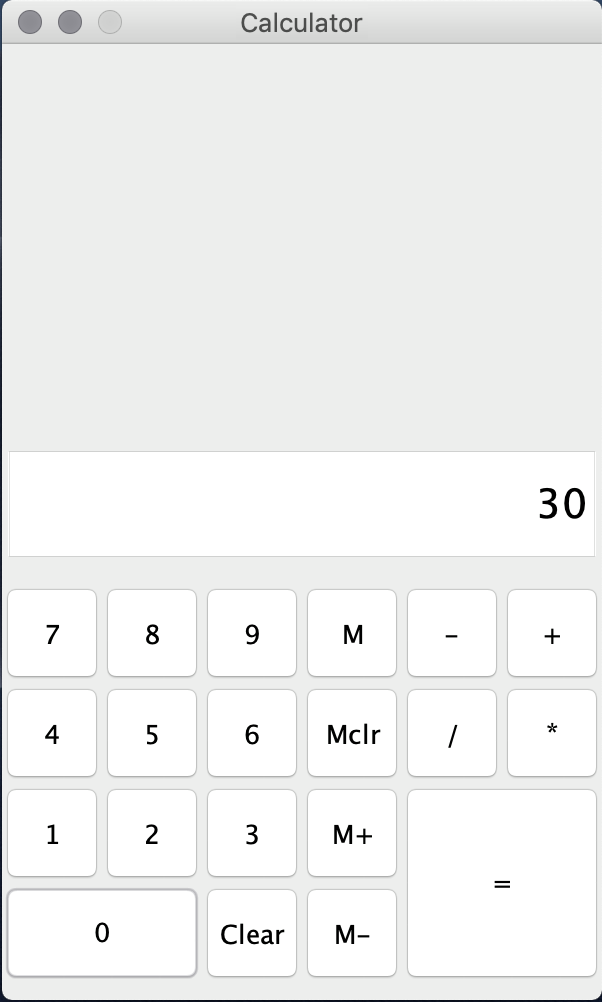
\includegraphics[width=0.4\textwidth, right]{calc_img.png}
	\caption{Calculator.}
	\label{fig:boat1}
\end{figure}



\end{document}          
